\documentclass[a4paper]{article}
\usepackage{amsmath}
\usepackage{fancyhdr}
\usepackage{graphicx}
\usepackage{pdfpages}
\pagestyle{fancy}
\lfoot{Andrew Martin}
\rfoot{10/8/2017}
\begin{document}
	\title{PDEs Assignment 2}
	\date{August 17, 2017}
	\author{Andrew Martin}
	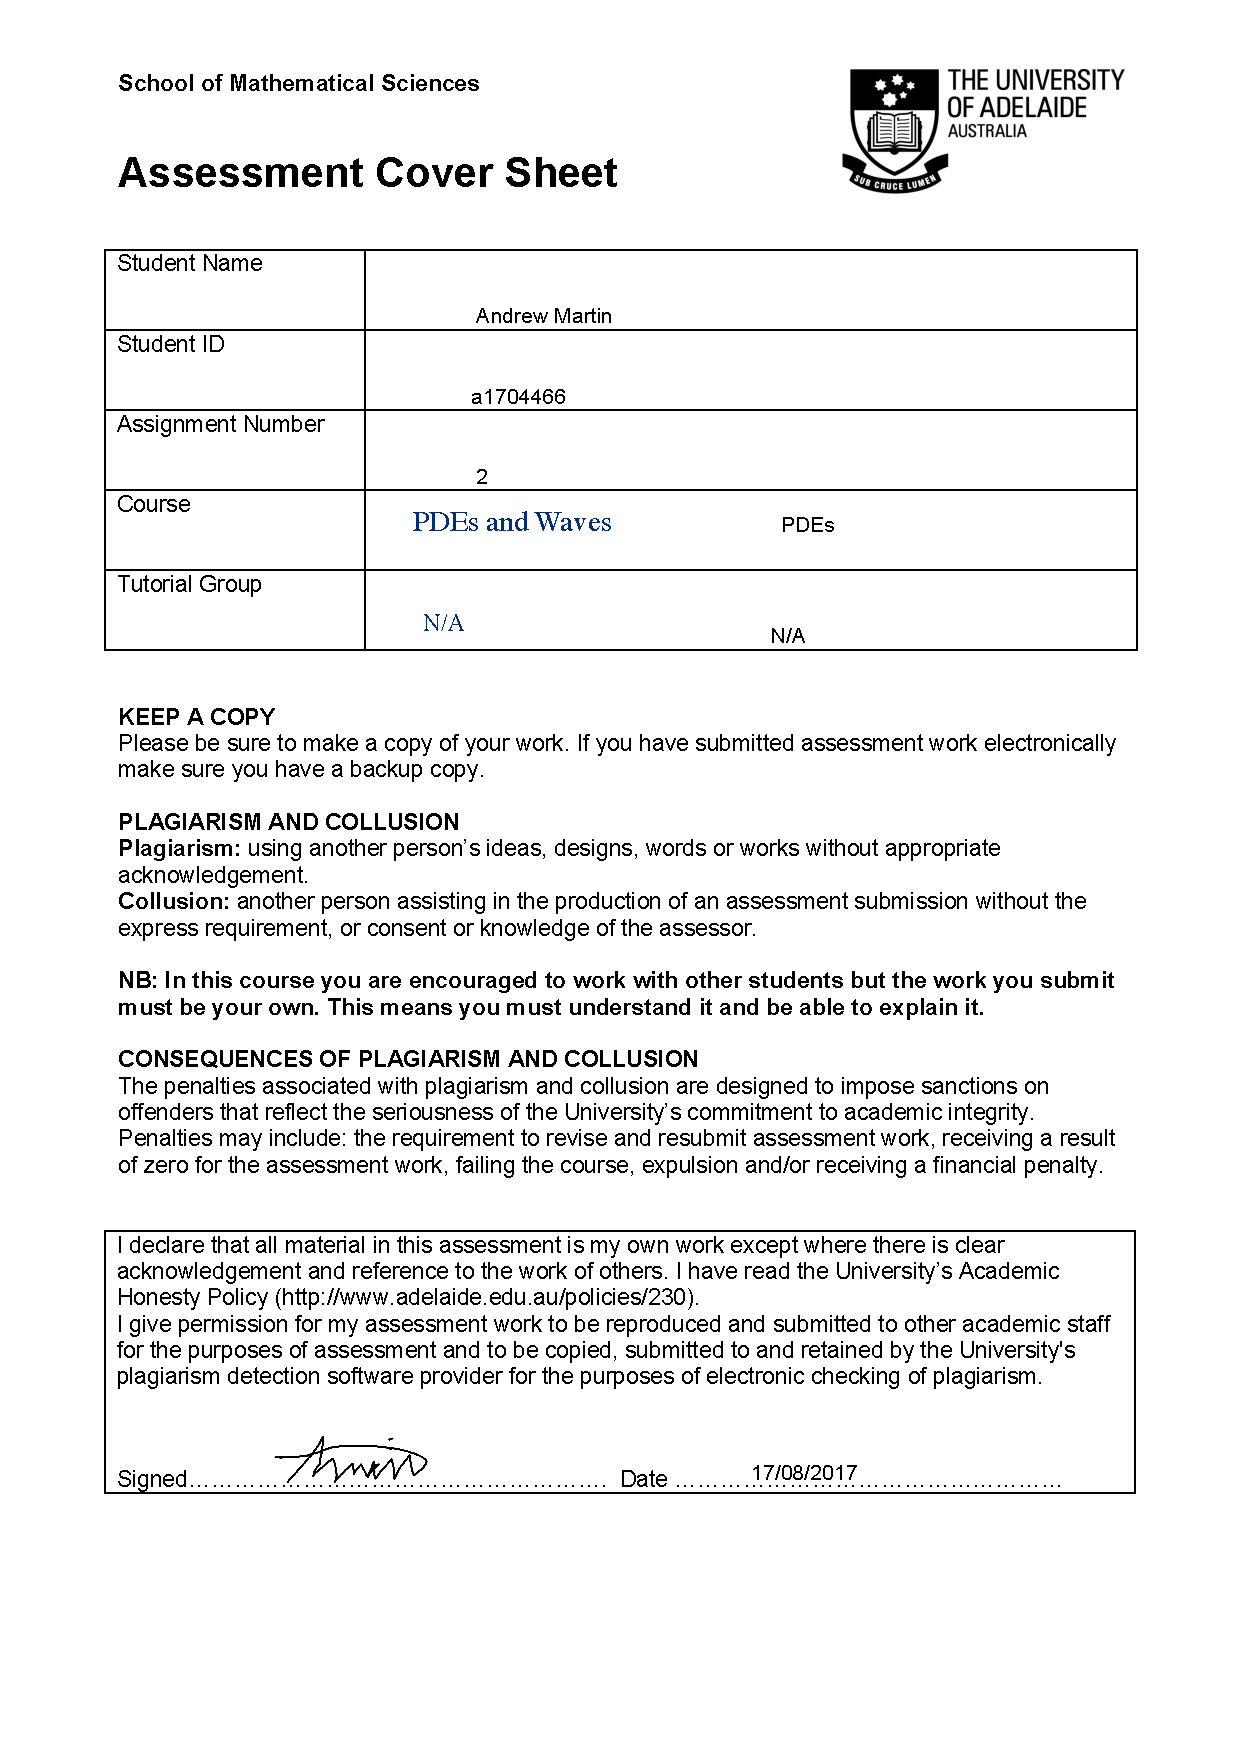
\includepdf[pages={1}]{coversheet.pdf}
	\maketitle
	
	Question 1:\\
	I was given a $\frac{4}{5}$ for mathematical writing in assignment 1.
	The mark was deducted due to a lack of explaining steps and derivations in some cases where the steps taken may have been unclear, and a formula similar to one derived in lectures was not fully explained.\\
	
	
	\newpage
	Question 2:\\
	Considering the PDE:
	$$\rho (x) \frac{\delta ^2 u}{\delta t ^2} = S_0(x)\frac{\delta ^2 u}{\delta x ^2}-\alpha(x)u-\beta(x)\frac{\delta u}{\delta t}$$
	The coefficients $\rho$, $S_0$ , $\alpha$, and $\beta$ are all functions of $x$. Show that separation of variables can only work if $\beta (x) = c\rho(x)$ for some constant $c$.
	
	
	\newpage
	Question 3:\\
	Spherically symmetric solutions $u(r,t)$, where r is radius from the origin, of the wave PDE in 3D:
	$$\frac{\delta ^2 u}{\delta t ^2}=c^2\left[\frac{\delta ^2 u}{\delta r ^2}+\frac{2\delta u}{r \delta r }\right]$$
	
	(a)\\
	Use separation of variables i.e. $u=R(r)T(t)$, to find an eigen-problem for the radial spacial structure $R(r)$.\\
	
	(b)\\
	Rearrange the ODE for $R(r)$ to write it in Sturm-Liouville form.\\
	
	(c)\\
	Show the the boundary conditions imply the linear operator in the Sturm-Liouville form is self-adjoint.\\
	
	(d)\\
	What does the infinity of real eigenvalues for this eigenproblem imply for the time dynamics $T(t)$?
	
	
	\newpage
	Question 4:\\
	Consider the regular Sturm-Liouville eigenproblem for $0 \leq x \leq 1$,
	$$u''+\lambda u = 0 \qquad u(0)=0 \qquad 3u(1)+u'(1)=0$$
	Verify the following properties via writing the eigenvalues as $\lambda = k^2$ where the values of k are the positive solutions of the transcendental equation $\tan(k)=\frac{-k}{3}$. (consider the graphs of $y=\tan(k)$ and $y=\frac{-k}{3}$).\\
	
	(a)\\
	There are an infinite number of eigenvalues with no largest one.\\
	
	(b)\\
	The $n$th eigenfunction has $n-1$ zeros over $0<x<1$ with boundary conditions that $u(0,t)$ and $u(1,t)$ are specified.\\
	
	(c)\\
	Write down the orthogonality condition for the eigenfunctions.\\
	Orthogonality of functions over the domain $[a,b]$  that for $m\neq n$:
	$$<v_m , v_n > =0$$
	I.e.
	$$\int_{a}^{b}v_m v_n r dx = 0$$
	In this case, the domain $[a,b]$ is the domain $[0,1]$. So with respect to some weight function $r(x)$ the orthogonality implies
	$$\int_{0}^{1}v_m v_n r dx = 0$$
	
	\newpage
	Question 5:\\
	Explore computationally approximating solutions $u(x,t)$ to the linear advection-diffusion PDE $u_t=-3u_x+u_{xx}$ on the domain $0<x<1$ with boundary conditions that $u(0,t)$ and $u(1,t)$ are specified.\\
	
	(a)\\
	Using Lagrange's remainder theorem, confirm that $f'(x) = \frac{[-f(x-h)+f(x+h)]}{2h} + Ch^2$ and find the expression for C.\\
	
	(b)\\
	The simplest discretised approximation to this advection-diffusion PDE is to have one grid point interior to the spatial domain: defining the grid $x_1 =0$, $x_2 =1/2$, and $x_3=1$, derive the approximate ODE for $u_2(t):=u(\frac{1}{2},t)=b$
	
	(c)\\
	Modify Algorithm 4.1 to computationally approximate solutions to the advection-diffusion PDE over time $0\le t \le 1$ with boundary values $u(0,t) = 0$ and $u(1,t) = sin(9t)$, and any reasonable initial condition of your choice.\\
	Submit code and graphical output here:
	
	
	
\end{document}